\documentclass[english,floatsintext,man]{apa6}

\usepackage{amssymb,amsmath}
\usepackage{ifxetex,ifluatex}
\usepackage{fixltx2e} % provides \textsubscript
\ifnum 0\ifxetex 1\fi\ifluatex 1\fi=0 % if pdftex
  \usepackage[T1]{fontenc}
  \usepackage[utf8]{inputenc}
\else % if luatex or xelatex
  \ifxetex
    \usepackage{mathspec}
    \usepackage{xltxtra,xunicode}
  \else
    \usepackage{fontspec}
  \fi
  \defaultfontfeatures{Mapping=tex-text,Scale=MatchLowercase}
  \newcommand{\euro}{€}
\fi
% use upquote if available, for straight quotes in verbatim environments
\IfFileExists{upquote.sty}{\usepackage{upquote}}{}
% use microtype if available
\IfFileExists{microtype.sty}{\usepackage{microtype}}{}

% Table formatting
\usepackage{longtable, booktabs}
\usepackage{lscape}
% \usepackage[counterclockwise]{rotating}   % Landscape page setup for large tables
\usepackage{multirow}		% Table styling
\usepackage{tabularx}		% Control Column width
\usepackage[flushleft]{threeparttable}	% Allows for three part tables with a specified notes section
\usepackage{threeparttablex}            % Lets threeparttable work with longtable

% Create new environments so endfloat can handle them
% \newenvironment{ltable}
%   {\begin{landscape}\begin{center}\begin{threeparttable}}
%   {\end{threeparttable}\end{center}\end{landscape}}

\newenvironment{lltable}
  {\begin{landscape}\begin{center}\begin{ThreePartTable}}
  {\end{ThreePartTable}\end{center}\end{landscape}}




% The following enables adjusting longtable caption width to table width
% Solution found at http://golatex.de/longtable-mit-caption-so-breit-wie-die-tabelle-t15767.html
\makeatletter
\newcommand\LastLTentrywidth{1em}
\newlength\longtablewidth
\setlength{\longtablewidth}{1in}
\newcommand\getlongtablewidth{%
 \begingroup
  \ifcsname LT@\roman{LT@tables}\endcsname
  \global\longtablewidth=0pt
  \renewcommand\LT@entry[2]{\global\advance\longtablewidth by ##2\relax\gdef\LastLTentrywidth{##2}}%
  \@nameuse{LT@\roman{LT@tables}}%
  \fi
\endgroup}


  \usepackage{graphicx}
  \makeatletter
  \def\maxwidth{\ifdim\Gin@nat@width>\linewidth\linewidth\else\Gin@nat@width\fi}
  \def\maxheight{\ifdim\Gin@nat@height>\textheight\textheight\else\Gin@nat@height\fi}
  \makeatother
  % Scale images if necessary, so that they will not overflow the page
  % margins by default, and it is still possible to overwrite the defaults
  % using explicit options in \includegraphics[width, height, ...]{}
  \setkeys{Gin}{width=\maxwidth,height=\maxheight,keepaspectratio}
\ifxetex
  \usepackage[setpagesize=false, % page size defined by xetex
              unicode=false, % unicode breaks when used with xetex
              xetex]{hyperref}
\else
  \usepackage[unicode=true]{hyperref}
\fi
\hypersetup{breaklinks=true,
            pdfauthor={},
            pdftitle={A Computational Perspective On Spatial Perspective Transformations: From Sensory Inference To Imagined Self-motion},
            colorlinks=true,
            citecolor=blue,
            urlcolor=blue,
            linkcolor=black,
            pdfborder={0 0 0}}
\urlstyle{same}  % don't use monospace font for urls

\setlength{\parindent}{0pt}
%\setlength{\parskip}{0pt plus 0pt minus 0pt}

\setlength{\emergencystretch}{3em}  % prevent overfull lines

\ifxetex
  \usepackage{polyglossia}
  \setmainlanguage{}
\else
  \usepackage[english]{babel}
\fi

% Manuscript styling
\captionsetup{font=singlespacing,justification=justified}
\usepackage{csquotes}
\usepackage{upgreek}

 % Line numbering
  \usepackage{lineno}
  \linenumbers


\usepackage{tikz} % Variable definition to generate author note

% fix for \tightlist problem in pandoc 1.14
\providecommand{\tightlist}{%
  \setlength{\itemsep}{0pt}\setlength{\parskip}{0pt}}

% Essential manuscript parts
  \title{A Computational Perspective On Spatial Perspective Transformations: From
Sensory Inference To Imagined Self-motion}

  \shorttitle{Vestibular Contributions to SPT}


  \author{Andrew W. Ellis~\& Fred W. Mast}

  \def\affdep{{"", ""}}%
  \def\affcity{{"", ""}}%

  \affiliation{
    \vspace{0.5cm}
          \textsuperscript{} Department of Psychology, University of Bern, Switzerland  }

  \authornote{
    \newcounter{author}
    Andrew W. Ellis \& Fred W. Mast, Department of Psychology. AE and FM
    planned and conducted the research; AE and FM performed the simulations
    and wrote the manuscript. Code for simulations is available at
    \url{https://osf.io/u26mq}.

                      Correspondence concerning this article should be addressed to Andrew W. Ellis, Fabrikstrasse 8, 3012 Bern, Switzerland. E-mail: \href{mailto:andrew.ellis@psy.unibe.ch}{\nolinkurl{andrew.ellis@psy.unibe.ch}}
                          }


  \abstract{Mental spatial transformations are considered to be an essential
cognitive ability. Recent research has indicated that the vestibular
network is involved in such mental spatial transformations. However, the
nature of this involvement remains unclear. We propose a computational
framework for the involvement of the vestibular system in cognition and
discuss this in the context of perspective transformations, which
require a simulated rotation of the self. We explore how the ability to
anticipate the sensory consequences of self-initiated actions might
underlie the ability to imagine body rotations. We approach this problem
by extending previous models of vestibular sensory inference to include
the ability to model the sensory consequences of self-initiated
movements, and discuss how this can be further extended to allow
mentally simulated rotations of the self. Our model is able to explain
various source of interference between simulations of self-rotation and
sensory inference.}
  \keywords{probabilistic graphical models, particle filter, embodied cognition,
vestibular cognition, spatial perspective taking, mental imagery, mental
simulation \\

    \indent Word count: X
  }

\usepackage[titles]{tocloft}
\cftpagenumbersoff{figure}
\renewcommand{\cftfigpresnum}{\itshape\figurename\enspace}
\renewcommand{\cftfigaftersnum}{.\space}
\setlength{\cftfigindent}{0pt}
\setlength{\cftafterloftitleskip}{0pt}
\settowidth{\cftfignumwidth}{Figure 10.\qquad}

\cftpagenumbersoff{table}
\renewcommand{\cfttabpresnum}{\itshape\tablename\enspace}
\renewcommand{\cfttabaftersnum}{.\space}
\setlength{\cfttabindent}{0pt}
\setlength{\cftafterloftitleskip}{0pt}
\settowidth{\cfttabnumwidth}{Table 10.\qquad}



\usepackage{amsthm}
\newtheorem{theorem}{Theorem}
\newtheorem{lemma}{Lemma}
\theoremstyle{definition}
\newtheorem{definition}{Definition}
\newtheorem{corollary}{Corollary}
\newtheorem{proposition}{Proposition}
\theoremstyle{definition}
\newtheorem{example}{Example}
\theoremstyle{remark}
\newtheorem*{remark}{Remark}
\begin{document}

\maketitle

\setcounter{secnumdepth}{0}



\section{Introduction}\label{introduction}

Adopting the spatial perspective of another person is an essential
cognitive ability, and plays a vital role in our ability to determine
possible actions of another person, and in order to coordinate joint
actions (Creem-Regehr, Gagnon, Geuss, \& Stefanucci, 2013, Pezzulo,
Iodice, Ferraina, and Kessler (2013)). Perspective taking is also
considered to be of fundamental importance for language comprehension
and communication (Beveridge \& Pickering, 2013), and social cognition
in general (Deroualle \& Lopez, 2014).\\
 A number of recent studies have demonstrated that the vestibular
system, which processes sensory signal relating to angular and linear
movements of the head, is involved in such spatial transformations
(Lenggenhager, Lopez, \& Blanke, 2008, Deroualle, Borel, Devèze, and
Lopez (2015), Falconer and Mast (2012), Gardner, Stent, Mohr, and
Golding (2016)). This is demonstrated in the form of interference
effects between mental transformations and concurrent sensory
stimulation. To date, however, there has little attempt to understand
the involvement of the vestibular system in higher-level cognitive
abilities in terms of the computational mechanisms. Consider the use of
deictic pronouns, such as \enquote{this} or \enquote{that} and
\enquote{left} or \enquote{right}. These terms only assume a meaning
relative to a certain frame of reference (FOR). For example, in a
dialogue between two speakers, the statement \enquote{I would like that
one}, or \enquote{I would like the one on the right} can only be
understood if both interlocutors are able to access the other's FOR with
respect to an external FOR. A further example that requires a similar
spatial transformation is when two people want to perform a coordinated
action, such as lifting a heavy object. This requires having knowledge
of the other's potential actions in order to adjust one's own actions,
and this again requires knowledge of the other's position within an
external FOR. A judgement about what kind of actions the other person
can perform requires an embodied simulation using a representation of
one's own body schema (Pezzulo et al., 2013) and giving an instruction
to another person thus requires running an embodied simulation in order
to infer what kind of motor commands the other person should perform
\textbf{{[}Blakemore and Decety, 2001; Wolpert et al., 2003; Jeannerod,
2006; Pezzulo et al., 2007, 2013; Dindo et al., 2011; Pezzulo,
2011a,b{]}}. But this again requires information about the addressee's
FOR relative to the external reference frame, and the difference between
the speaker and the addressee's egocentric reference frames. Perspective
taking can be conceived of as a aligning a representation of one's body
with that of another person in order to access spatial information from
a viewpoint other than one's own egocentric viewpoint. In order to
achieve this alignment, one must perform translations and rotations of
one's own egocentric reference frame. Processing translations and
rotations of the head and body is the core domain of the vestibular
system, and thus is of particular interest for research into mental
spatial transformations. Spatial transformations in 6 dimensions
(translation along 3 axes, and rotations around 3 axes) are highly
complex, and non-linear, and it has been proposed that the brain adopts
the strategy of simulating motion of the body through space in order
achieve a desired target position {[}CITATION{]}. This effectively
amounts to a running a simulation of dynamical system, consisting of
simulated limb movements and the resulting sensory consequences. Figure
\ref{fig:spt-schematic} (a) shows a simple scenario in which a speaker
wants to tell an addressee, standing opposite, to pick something up from
the floor. The speaker must determine the most suitable action by
embodied simulation, given the addressee's position relative to the
external object, and in order to achieve this goal, the speaker must
align himself with the addressee, so that he can use his own
body-centred FOR. In this example, alignment with the addressee's
reference frame consists of a forwards translation and a rotation around
the vertical axis. This can be described as an imagined movement, in
which the goal is achieve a specific position.

\begin{figure}
\centering
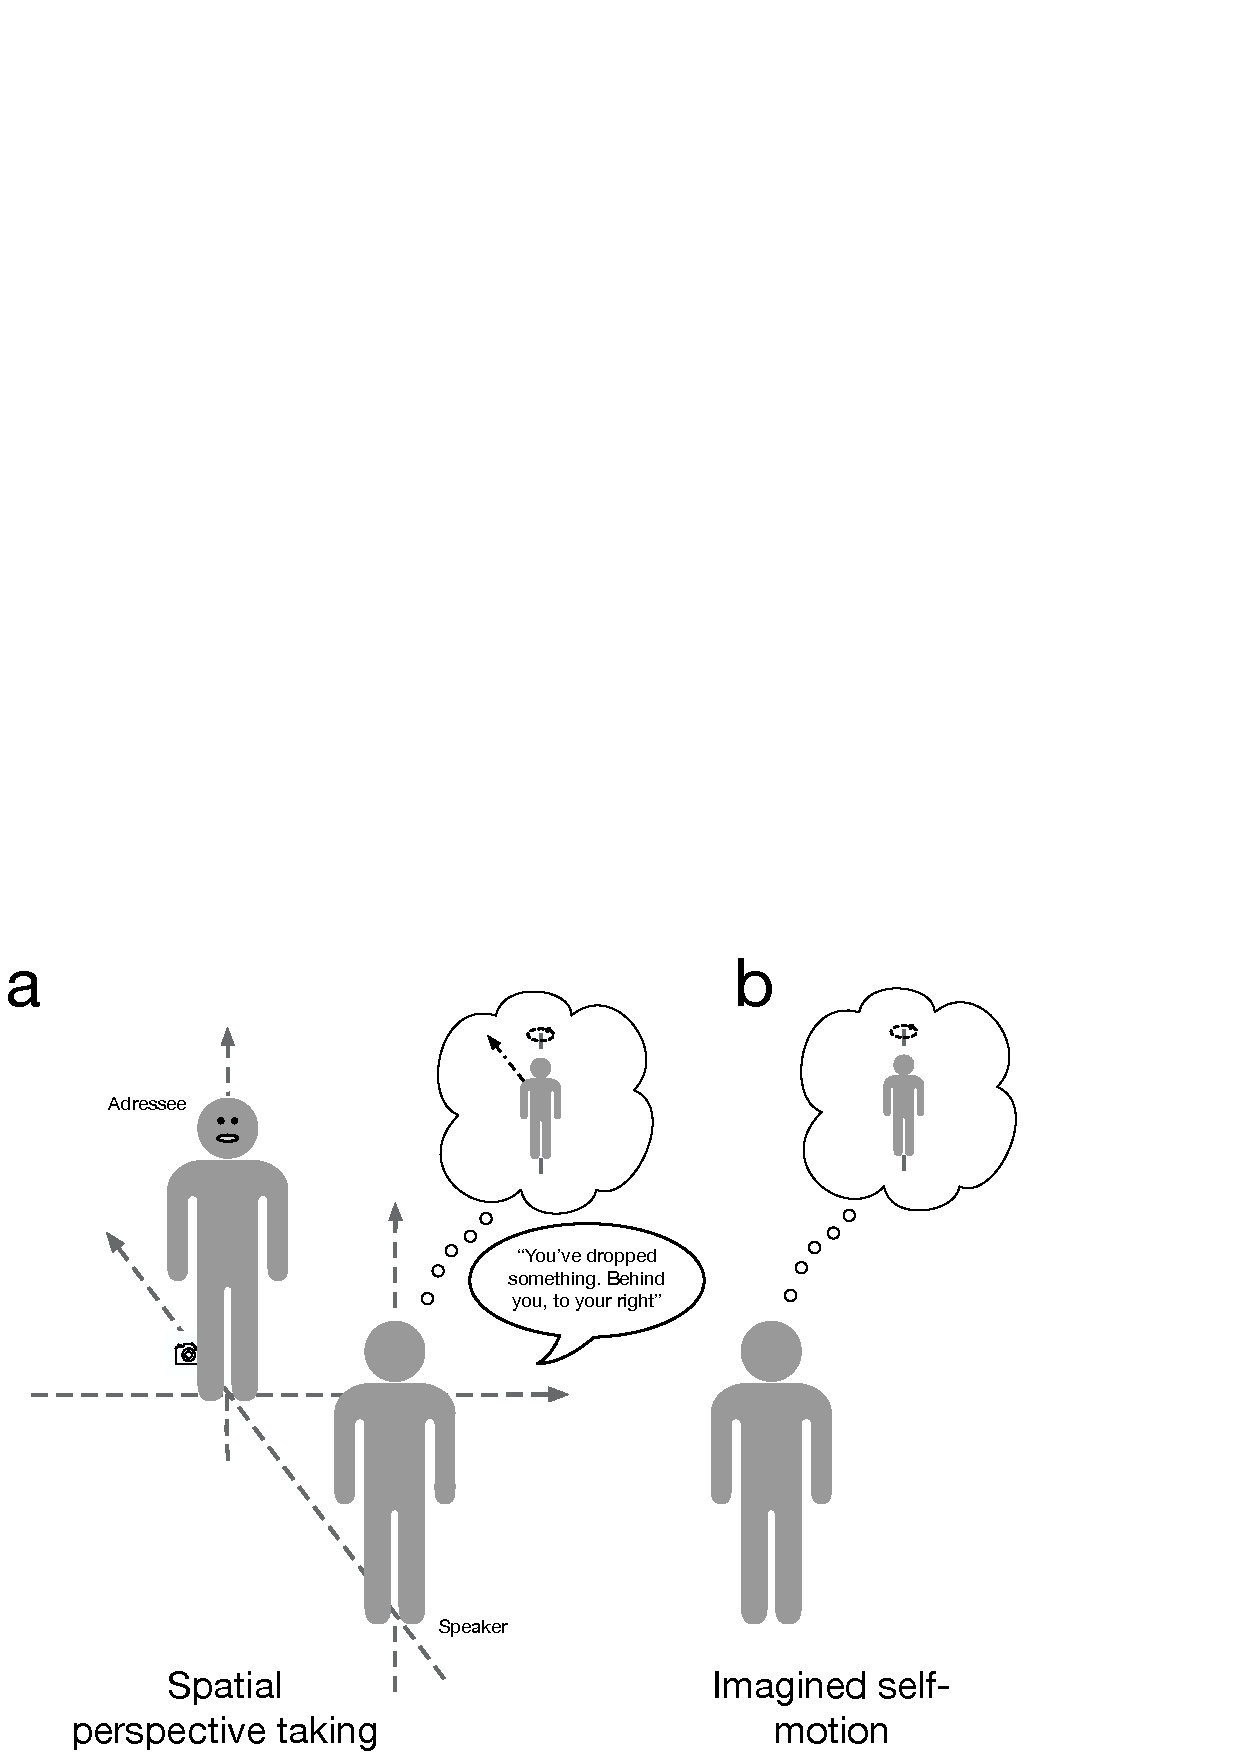
\includegraphics{diagrams/fig-1-common-process.pdf}
\caption{\label{fig:spt-schematic}Perspective taking and imagined
self-motion involve spatial transformations of a representation of the
self. (a) If a speaker's goal is to take the perspective of an
addressee, he must first solve the inverse problem of determining the
appropriate action, and then run a forwards simulation in order to
perform a translation and rotation of his own egocentric reference
frame. These operations can be viewed as imagined movements.(b)
Focussing on imagined rotation around the vertical axis allows us to
simplify the problem, and highlights the fact that perspective taking
and mental imagery involve common computations.}
\end{figure}

In order to do this, the speaker must first determine what type of
movement to perform. This means that in order to know what to simulate,
the speaker must first work backwards from the desired outcome, and
infer the actions that are most likely to lead to that outcome (Hamrick
\& Griffiths, 2014). In the field of motor control, this is known as the
inverse problem (Wolpert \& Kawato, 1998). In order to achieve the
desired position, the motor commands can then be simulated, and the
expected sensory consequences can be estimated; this is known as the
forward problem. Figure \ref{fig:spt-schematic} (b) shows that if the
goal is to deliberatively simulate the perceptual experience of rotation
around the body's vertical (yaw) axis, rather than project a
representation of one's body onto a target, the problem is simplified;
the actor can perform forward inference without the need to determine
the optimal motor action. As demonstrated by Penny, Zeidman, and Burgess
(2013), these computations can be performed in a common probabilistic
model. Interestingly, this has been discussed in the context of
reinforcement learning, and planning in humans has been described as
reverse inference (Botvinick \& Toussaint, 2012). Further, (Pickering \&
Clark, 2014) discuss the relationship between control-theoretic notions
of inverse/forward models, known collectively as internal models, and
and more general concepts of a generative model in a hierarchical
Bayesian framework. Simulating the behaviour of a dynamical system using
a forward model requires a generative model of the system.

The aim of this paper is to specifically investigate the generative
model that may be used for mental spatial transformations. The ability
to run embodied simulations is often claimed to be grounded in the
relevant sensorimotor circuits, and we claim that the vestibular system
is ideally suited to investigate this connection, because the generative
models used by the vestibular system for dynamic sensory inference have
been extensively investigated using approaches from optimal control
theory, and more recently, dynamic Bayesian inference (Oman, CITATIONS,
MacNeilage, Ganesan, \& Angelaki, 2008).

The vestibular system faces a number of challenges in interpreting the
sensory measurements provided by the semi-circular canals (SCC) and
otolith organs. On the one hand, these signals are very noisy, and
ambiguous; the otoliths respond both to translations and tilt of the
head relative to gravity, and in order to disambiguate between
translation and tilt, the brain must perform sophisticated computations.
The emerging picture is that the nature of these computations is
probabilistic, and that the brain makes use of strong prior beliefs in
order to interpret these sensory signals {[}Mittelstaedt, etc{]}. A
further challenge faced by the vestibular system is that it needs to
distinguish between sensory signals that are the result of active
motion, and those resulting from external forces (Cullen, Brooks, \&
Sadeghi, 2009, Cullen (2014)). The ability to distinguishing re-afferent
from ex-afferent sensory signals is an essential capability of all
organisms that move actively (Crapse \& Sommer, 2008).

Furthermore, the apparent connection between mental imagery and
predictive processing has repeatedly been alluded to (Moulton \&
Kosslyn, 2009, Clark (2012), Gambi and Pickering (2015)), and Grush
(2004) claims that mental imagery is performed by emulator circuits
implementing a forward model. These ideas can also be addressed from a
computational point of view in the context of dynamic Bayesian
inference, where there are multiple roles for sensory predictions, over
different time scales. This was recently discussed by (Tian \& Poeppel,
2012) in the context of imagined speech. The putative link between
predictive processing and higher cognitive processing has a firm basis
in predictive processing accounts of sensory inference {[}Friston{]}.
The predictive processing framework has been applied to almost all
sensory modalities {[}CITATIONS: pain, proprioception, auditory ,
visual, etc.{]}, and the picture that has emerged in recent years is
that the brain employs sophisticated inference algorithms in order to
\enquote{interpret} the stream of incoming sensory data. The brain seems
to be actively engaged in formulating hypotheses, and testing these on
sensory data; this has been extended to the concept of active inference
{[}Friston{]}, in which an agent attempts to either change it's internal
model of world, or to intervene on the world in order to fulfill sensory
predictions.

We claim that the vestibular modality is particularly well-suited to
investigating predictive processing at multiple hierarchical scales,
from the lowest levels of sensory inference to higher levels, where
goals, intentions and beliefs of the organism become relevant. A case in
point is the study by Wertheim, Mesland, and Bles (2001), who provided
evidence that participants' perceptions of tilt induced by vestibular
stimulation are shaped to a large extent by the beliefs about possible
motions they formed prior to taking part in the experiment.

Interference effects between higher-level cognitive processes, such as
SPT and mental imagery, and sensory inference, are thought to occur as a
result of shared circuitry (Deroualle \& Lopez, 2014, Nigmatullina et
al. (2015)). However, the precise nature of such interactions, and what
exactly might be shared, is left unspecified. At first glance, it appear
unlikely that such interference should be possible, as low levels of
vestibular processing appear to be cognitively impenetrable
{[}CITATION{]}. In particular, Nigmatullina et al. (2015) found that the
onset of the vestibulo-ocular reflex (VOR) was earlier when the
direction of an imagined self-rotation was congruent with the direction
of a subsequently experienced rotation. The VOR, however, must be
susceptible to the influence of intentions and goals; for example, if a
person intends to fixate a target during a movement, the VOR should be
cancelled. Thus, seemingly reflexive, and impenetrable, motor actions
require a large amount of flexibility based on top-down information.
Even accepting the fact that low level sensorimotor processing may be
more cognitively penetrable than previously thought, the fact that
imagining a rotation of the self should have an effect on a person's
ability to detect rotations, or to discriminate between directions of
rotation, still requires an explanation.

\begin{quote}
NOTE: we need to include all studies demonstrating interference,
especially in the direction cognition -\textgreater{} inference
(Nigmatullina effect)
\end{quote}

Ellis and Mast (2017) recently claimed that the types of interference
effects might arise as a result of cognitive processing exerting an
influence on circuits performing sensory inference via shared
higher-level priors. In particular, the interference described by
Nigmatullina et al. (2015) looks like an effect of a bias in the sensory
discrimination task. Although vestibular perceptual thresholds have been
extensively investigate for yaw rotations (Grabherr, Nicoucar, Mast, \&
Merfeld, 2008; Merfeld, 2011), the methods used for estimating
thresholds require unbiased responding by the participants. There have
no investigations of biasing effects on yaw rotations.

In this paper, we pursue the claim that interference should be
investigated as a bias, and we attempt to explain the grounding of
higher level cognitive abilities in the computations performed by
low-level sensory circuits in the service of dynamic real-time
interactions with the world.

Kwisthout, Bekkering, and Rooij (2016) make the point that predictive
processing accounts are situated at low levels in the processing
hierarchy, usually at the level of sensory inference or at the level
describing kinematics.

In this paper, we address this issue by starting from a model developed
for low-level sensory inference, incorporating basic abilities to
predict sensory consequences of movement based on knowledge about the
kinematics, and extending this to account for interactions between
thought processes, operationalized as mental simulations of sensorimotor
experience, and sensory processing.

Battaglia, Hamrick, and Tenenbaum (2013) addressed the idea that the
higher level cognitive ability to perform mental rotation are grounded
in the circuits performing sensory inference. We claim that if
vestibular cognition is grounded in sensory inference, and that this is
to be experimentally studied by analyzing interactions between thought
and sensory inference, then it is vital that this be carried within the
constraints of a theoretical (computational) framework. A suitable
formalism for this is the framework of probabilistic graphical models
(Pearl, 1988, Koller and Friedman (2009)), and within this framework,
interactions between thought and perception can be modelled as effects
of higher level priors and hyperpriors on inference at a computational
level. Investigating inference at the level of algorithmic
implementations might provide further insight.

Probabilistic graphical models are able to represent hierarchically
structured knowledge (Kwisthout et al., 2016, Griffiths, Vul, and
Sanborn (2012)), which is required for Bayesian models of cognition
(Tenenbaum, Kemp, Griffiths, \& Goodman, 2011, Lucas and Griffiths
(2010)). This approach has been used to model concept learning (Kemp,
Perfors, \& Tenenbaum, 2007), inductive biases in reasoning, in
cognitive models of development (A. Perfors, Tenenbaum, Griffiths, \&
Xu, 2011), language (Goodman \& Frank, 2016) and social cognition
(Baker, Saxe, \& Tenenbaum, 2009).

In this paper, we focus specifically on the role of the vestibular
system for spatial perspective transformations, and we draw the link
between probabilistic computations performed by the vestibular system,
and the brain's ability to run mental simulations for the purpose of
adopting the perspective of another person.

We proceed by introducing recent models of Bayesian inference for
real-time, dynamic sensory processing of vestibular data, based on
particle filters (Laurens \& Droulez, 2007, Karmali and Merfeld (2012)),
and we re-frame these as probabilistic graphical models. This allows us
to investigate the generative model separately from the algorithm used
for inference, and we then extend the basic model for sensory inference
in order to focus specifically on the ability to model the consequences
of self-initiated, active movements. This is an implementation of the
idea that information about motor commands are projected to sensory
areas by means of an efference copy, based on which a forward model then
computes the sensory consequences. Our aims are to:

\begin{enumerate}
\def\labelenumi{\arabic{enumi})}
\tightlist
\item
  identify various forms of predictive processing in the context of
  dynamic sensory processing.
\item
  identify various sources of interference between higher-level
  cognition and lower-level sensory processing.
\item
  provide suggestions for future research aiming to investigate the
  connections between cognitive and sensory processing.
\end{enumerate}

Following Karmali and Merfeld (2012), we focus on one specific type of
head movement, a rotation of the head about the yaw axis, and discuss
this in the context of the probabilistic computations that are performed
when the goal is to:

\begin{enumerate}
\def\labelenumi{\arabic{enumi})}
\tightlist
\item
  infer motion caused by external events
\item
  infer the consequences of one's own actions.
\end{enumerate}

\section{Dynamic Bayesian models for sensory
inference}\label{dynamic-bayesian-models-for-sensory-inference}

\subsection{Previous work}\label{previous-work}

Whereas early models of vestibular sensory processing were inspired by
control theory (Borah, Young, \& Curry, 1988, Merfeld, Zupan, and
Peterka (1999)), several recent studies have described vestibular
sensory processing as dynamic Bayesian inference (Laurens \& Droulez,
2007, MacNeilage et al. (2008), Karmali and Merfeld (2012)). Selva and
Oman (2012) provide a recent review of the relationship between optimal
observer models and models that employ Kalman filtering, and show that
these are largely equivalent. Both Karmali and Merfeld (2012) and
Laurens and Droulez (2007) described vestibular sensory inference in
terms of particle filtering, which is a particular algorithm that can be
used to perform inference in state-space models. (Doucet, Godsill, \&
Andrieu, 2000, Doucet and Johansen (2009)). Using their model, Laurens
and Droulez (2007) were able to simulate perceptual responses to
centrifugation and off-vertical axis rotations. A well-known phenomenon
of vestibular perception is velocity storage, which is defined as the
slower decay of perceptual and oculomotor responses, relative to the SCC
afferent responses (Raphan, Matsuo, \& Cohen, 1979), \textbf{{[}Robinson
1977{]}}. This is generally seen as evidence for the existence of an
internal model in the processing of vestibular signals. Karmali and
Merfeld (2012) focused on one-dimensional angular velocity during yaw
rotations; their model was able to explain the phenomenon of velocity
storage as a consequence of particle filtering, with the time constant
of velocity storage depending on the noise of the sensory afferent
signals.

\subsection{Generative model for sensory
inference}\label{generative-model-for-sensory-inference}

We proceed by providing a brief introduction to the concept of
state-space models, and particle filtering, which is a particular
algorithm that can be used to perform inference in state-space models.
State-space models can be seen as special cases of more general dynamic
probabilistic graphical models (Bishop, 2006; Murphy, 2012), and are
suitable for modelling the time-varying behaviour of a system in terms
of a latent, unobservable process and noisy measurements.

\subsubsection{Dynamics/kinematics}\label{dynamicskinematics}

For example, consider trying to estimate the velocity and position
during a leftward head turn. In this case, the latent process provides a
model of the kinematics of the system, and the measurement model
describes how the afferent SCC signals are generated, dependent on the
kinematics.

The SCC signals are considered to be proportional to the angular
velocity of the head within a frequency band of approximately 0.1 -- 10
Hz, which constitutes the range of natural head movements (Carriot,
Jamali, Chacron, \& Cullen, 2014; Grabherr et al., 2008). These
measurements, however, are contaminated by Gaussian noise, which is
determined by characteristics of the sensory organs. Figure
\ref{fig:head-turn-data} shows a sequence of noisy measurements during a
two-second leftward turn of the head. The acceleration generating the
movement is sinusoidal, given for each time step \(t\) by
\(Asin(2\pi t/T)\), where \(A\) is the amplitude of the movement,
\(T = 1/f\) is the duration of the movement, and \(f\) is the frequency.
This acceleration results in a half-cycle cosine velocity profile, with
a peak velocity \(\omega_{peak} = AT/\pi\) and a final angular position
\(\theta_{final} = AT^2/2\pi\). Particle filtering provides a means of
filtering out the noise inherent in the measurements, and allows
estimation of evolution of the unobservable, latent state variables.

\begin{figure}
\centering
\includegraphics{generated-figures/head-turn-data-1.pdf}
\caption{\label{fig:head-turn-data}Sensory measurements obtained during a
short leftward head turn. The goal is to infer the latent angular
velocity and position, based on the noisy measurements.}
\end{figure}

\subsubsection{State-space notation}\label{state-space-notation}

The dynamics of the system can be modelled by the evolution of the 3-d
latent state variable\footnote{A state-space model reduces an
  n\textsuperscript{th} order difference equations (in discrete time) to
  n first-order difference equations.}, representing the position and
its derivatives, velocity and acceleration, as a first-order Markov
process, where the state at each time point \(t\) depends only on the
previous state at time \(t-1\). This is referred to as the process
model. Estimating the position \(\theta\), velocity \(\omega\) and
acceleration \(\alpha\) in discrete time requires writing the kinematic
equations as a set of first order difference equations.

\[ \theta_t = \theta_{t-1} + \omega_{t-1} \Delta t + \alpha_{t-1} \frac{1}{2} \Delta t^2 \]
\[ \omega_{t} = \omega_{t-1} + \alpha_{t-1} \Delta t \]
\[ \alpha_t = \alpha_{t-1} \]

This model assumes a constant acceleration. These kinematic equations
form a linear model, and could optionally be written in matrix notation.
For simplicity, we retain the current notation. Next, we consider the
measurements at each time step \(t\) as depending only on the current
state. This simply implements the idea that the sensory signal depends
only on the current head velocity. The above equations represent the
expected values of the state and observation variables. In order to
complete the generative model, we require a description of the
stochastic nature of the dependencies. We model both process and
measurement noise as being normally distributed, leading to the
following linear Gaussian state-space model:

\[ x_t = f(x_{t-1}, \epsilon) \] \[ y_{t} = g(x_t, \delta) \]
\[ \epsilon \sim N(0, \sigma^2_\epsilon) \]
\[ \delta \sim N(0, \sigma^2_\delta) \]

where the state variable \(x_t\) consists of the position \(\theta_t\),
velocity \(\omega_t\) and acceleration \(\alpha_t\), and \(y_{t}\)
denotes the sensory measurement. \(\epsilon\) and \(\delta\) are
zero-mean Gaussian noise terms with variances \(\sigma^2_\epsilon\) and
\(\sigma^2_\delta\). These refer to the process and measurement noise,
respectively. The process noise represents the uncertainty in the
dependence of the current state on the previous state; under the
constant velocity assumption, the process noise must be large enough if
the model is to allow for change in velocity due to unmodelled
acceleration. Note that the measurement noise is a model of the noise
characteristics of the sensor, and not a physical property of the sensor
itself. The function \(f\) and \(g\) represent the process transition
function and the measurement function, respectively.

Figure \ref{fig:graphical-model-inference} shows a representation of a
state-space model as a graphical model, unrolled over multiple time
steps. The state evolves according to the process model, with the
measurements at each time step being generated according to the
measurement model. The 3-dimensional latent state variable is unshaded,
to indicate that it cannot be observed, wheres the observed sensory
measurements are shaded. Given a generative model, we can apply various
sampling algorithms, either in order to run a Monte Carlo simulation by
sampling from the prior without incorporating any observed variables, or
to perform inference, by conditioning on observed variables. After a
brief discussion particle filtering, an inference algorithm often used
to infer the values of the latent state variables, we will introduce our
extension to the model that will allow a prediction of the consequences
of active movements.

\begin{figure}
\centering
\includegraphics{diagrams/dynamic-belief-network-inference-1.pdf}
\caption{\label{fig:graphical-model-inference}Graphical model for inferring
the 2-dimensional state \(x\), consisting of angular velocity and
position, based on noisy sensory measurements \(y\).}
\end{figure}

\subsection{Bayesian inference using particle
filtering}\label{bayesian-inference-using-particle-filtering}

We give a brief overview of particle filtering, a sequential Monte Carlo
algorithm for performing approximate Bayesian inference in a graphical
model. We describe a simple bootstrap particle filter, concentrating on
those aspects most relevant for this study. For a more thorough
treatment, see Doucet et al. (2000) and Doucet and Johansen (2009).
Speekenbrink (2016) provides a recent review with applications in
psychological research. Particle filtering proceeds by recursively
estimating the distribution of the current state, \(P(x_t | y_{1:t})\),
as a function of its parent nodes, conditional upon the sequence of
measurements \(y_{1:t}\). The distributions are represented by a
collection of discrete weighted samples, known as particles.

The general procedure for recursive Bayesian inference is to start from
an initial prior distribution, and the to perform alternating prediction
and updating steps. In other words: first, a hypothesis about the
expected state is generated, and then this hypothesis is tested by
evaluating how well it predicts the data. The algorithm starts with a
prior distribution of the particles, and at each subsequent time step,
proceeds by first sampling from the proposal distribution
\(P(x_t | y_{1:t-1})\), which is based on the specific choice of
transition function. Next, during the updating step, the current
measurement is incorporated by evaluating the likelihood,
\(P(y_t | x_t)\), which gives the probability of observing the
measurement for each individual particle. The particle are then assigned
an importance weight, based on how well they predicted the measurement.
A common problem in sequential Monte Carlo methods is that the particle
weights tend to become very small over time; this is known as the
degeneracy problem. In order to counteract this, multinomial resampling
is performed when effective sample size falls under a threshold. A new
set of particles is then chosen by weighted sampling with replacement,
which each particle's probability of being selected given by its
importance weight. Resampling ensures that only particles with a
relatively large probability of \enquote{explaining} the observations
are maintained. This introduces flexibility in the algorithm's method
for incorporating evidence into its beliefs about the latent states.

Figure \ref{fig:particle-filter-explained} shows a visualization of the
computations performed by a particle filter at each time step, in order
to track the angular velocity. Initially, the particles are propagated
forwards in time according to the proposal distribution. They are
equally weighted, indicated by their diameters. During the update step,
the particle are re-weighted, with each particle's weights reflecting
how well it explains the measurement. This is visualized by the change
in diameter; those particles lying close to the observation (sensory
input from the horizontal canal) have a larger diameter. After
resampling, the new set of particles is pulled towards the measurement,
and the weights are reset. This adjustment toward the observation
depends on both the process noise, and the modelled sensor noise. The
uncertainty of the belief, as indicated by the particle cloud's standard
deviation (light grey lines), increases at every prediction step, and
subsequently decreases after updating. This cycle of prediction,
updating and resampling ensures that the collection of particles comes
to represent the \enquote{true} posterior distribution, by eliminating
those particles with low weights. The particle filter represents all
beliefs in the form of probability distributions; the mean and variance
of the belief distribution can be computed at each time step, and the
logarithm of the weights \(log(\frac{1}{N}\sum^N_{i=1}w_i)\), averaged
over all \(N\) particles, may be summed over all time steps in order to
compute the log-likelihood
\(\sum^T_{t=1}\Big[log(\sum^N_{i=1}w_i) - log(N)\Big]\), which can be
used in order to evaluate how well the model was able to fit the sensory
evidence. The summed log-likelihood can be used for parameter estimation
in extensions of the basic particle filtering algorithm (Andrieu,
Doucet, \& Holenstein, 2010).

\begin{figure}
\centering
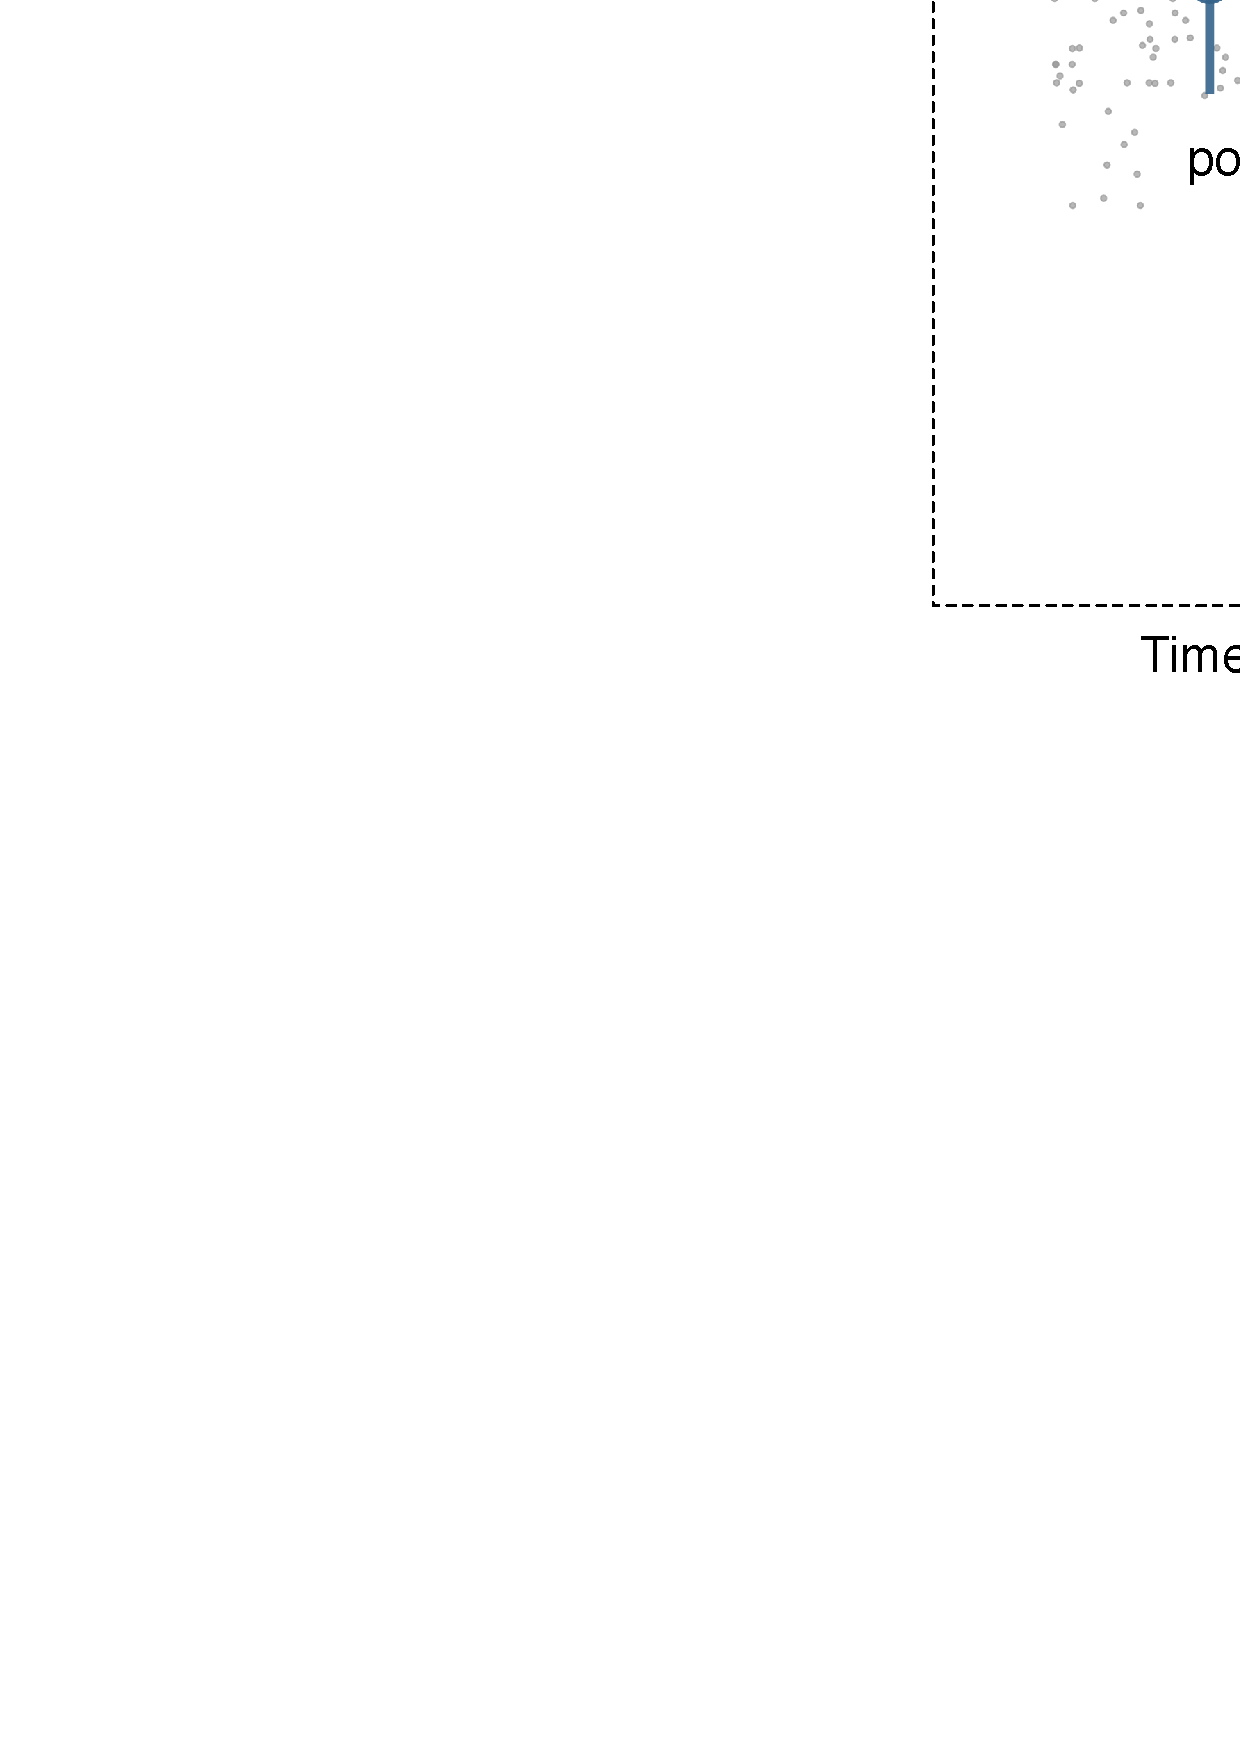
\includegraphics{diagrams/figure-particle-filter-explained.pdf}
\caption{\label{fig:particle-filter-explained}Particle filter computations
performed at every time step. The cloud of particles (grey circles)
represents the current belief state. Initially, message=FALSE,
warning=FALSE, a prediction is made for each particle by sampling from
the proposal distribution, which is determined by the agent's kinematic
model. This is equivalent to sampling from the prior distribution. Then,
during the updating step, an observation is obtained (shown as a black
diamond). Each particle is assigned an importance weight, according to
how well it explains the observation. Each particle's diameter reflects
its importance weight. Subsequently, a new set of particles is formed by
weighted multinomial resampling, with each particle's probability of
being chosen proportional to its importance weight. The particle cloud's
mean and standard deviation are shown as light grey circles and lines.
This resulting cloud of particles represents the posterior distribution.
This posterior subsequently forms the prior distribution for the next
time step.}
\end{figure}

\begin{figure}
\includegraphics[width=14.65in]{diagrams/particle-filter-algorithm} \caption{Particle filter computations performed at every time step.}\label{fig:particle-filter-algorithm}
\end{figure}

Figure \ref{fig:3d-statespace-fits} (a) shows the result of applying the
particle filtering algorithm to the graphical model depicted in Figure
\ref{fig:graphical-model-inference} and simulated measurements, in order
to infer the velocity and position during a two-second leftward head
turn. The acceleration is also inferred, but is not of interest.

The measurements are shown as circles, and the true velocity that
generated the data is shown as a dotted line. This velocity is the
result of an external force being applied. The solid lines depict the
mean estimates, and the shaded areas show the \(95\%\) credible
intervals. The model is able to estimate the latent state despite making
the assumption that the acceleration is constant. It does this by
allowing for random changes in acceleration by letting the process noise
be sufficiently large. Note that both position and velocity estimates
lag the true values; this is due the fact that the acceleration is
expected to be constant, and thus the system is slow to react to
changes. The estimation can be improved by increasing the process noise.
Figure \ref{fig:3d-statespace-fits} (b) shows the resulting estimates.
Whilst the lag is reduced, a consequence of increasing the process noise
is that the measurements are given more weight, resulting in a tendency
to over-fit the noise in the measurements. The constant velocity (random
acceleration) model is unable to capture the underlying smooth
trajectory of the velocity and position, instead showing random jumps in
the velocity estimate.

\begin{figure}
\centering
\includegraphics{generated-figures/3d-statespace-fits-1.pdf}
\caption{\label{fig:3d-statespace-fits}(a) Particle filter with a 3-d state
space model for inferring velocity and position during a two-second head
turn. (b) The same particle filter with increased process noise.}
\end{figure}

\section{Extension allowing the prediction of active
movements}\label{extension-allowing-the-prediction-of-active-movements}

During sensory inference the measurements are incorporated, and and a
posterior estimate of the latent state is obtained by updating the prior
with the likelihood. The underlying kinematic model thus relies on the
sensory data to inform its estimates. This model can be used in order to
track the behaviour of a dynamic system by including the acceleration as
a latent state, it is purely data-driven, and does not include any means
of incorporating an active prediction of the kinematics. Thus, it cannot
explain top-down expectations or biases. This form of anticipation is
not the same as the 1-step ahead predictions made during inference, but
rather implements higher level prior beliefs about the direction of
movement. For example, imagine seeing that someone is going to push you.
You can use this information, derived from the visual modality, in order
prepare yourself in order to compensate for this. However, you do not
want to act too early, but rather wait until you are actually moving.

\begin{quote}
While this model is perfectly suitable for sensory inference, for the
task of predicting the sensory consequences of self-initiated
movemenents, the model is inadequate, as it does not allow including
further knowledge about kinematics, which can be used to improve the
proposal distribution. This knowledge is obtained by means of an
efference copy of executed or planned motor commands, which is sent to a
forward model. The forward model must then translate the information
from the efference copy in a format that is suitable for the sensory
system.
\end{quote}

An obvious way of including this is the mechanism that allows one to
predict the sensory consequences of self-initiated movement via an
efference copy. In state-space models, this is implemented as a control
input \(u\), which extends the graphical model shown in Figure
\ref{fig:graphical-model-inference}. In this model, the estimated
acceleration is replaced by an known acceleration signal. This
capability to predict the consequences of self-initiated movements is
essential in order to distinguish re-afference from ex-afference - the
system has knowledge about how it moves, and can use this to predict the
sensory consequences. A further benefit of including a control input is
that the model can now be used in order to run counterfactual
simulations of the dynamic behaviour of the system for various types of
movements.

We implement the control in the following manner: during an active head
movement, the model generates a sequence of control signals \(u_{1:T}\).
For example, during a leftward head turn, using the sinusoidal
acceleration profile shown in Figure \ref{fig:head-turn-data}, the
acceleration is given by \(Asin(2\pi t/T)\). Assuming the model has full
knowledge about the onset of movement, and the type of movement
(sinusoidal head turn), the model requires information about the
frequency, \(f = 1/T\), amplitude, \(A\), and direction, which is given
by the sign of the amplitude.

Figure \ref{fig:graphical-model-control} shows the resulting graphical
model.

\begin{figure}
\centering
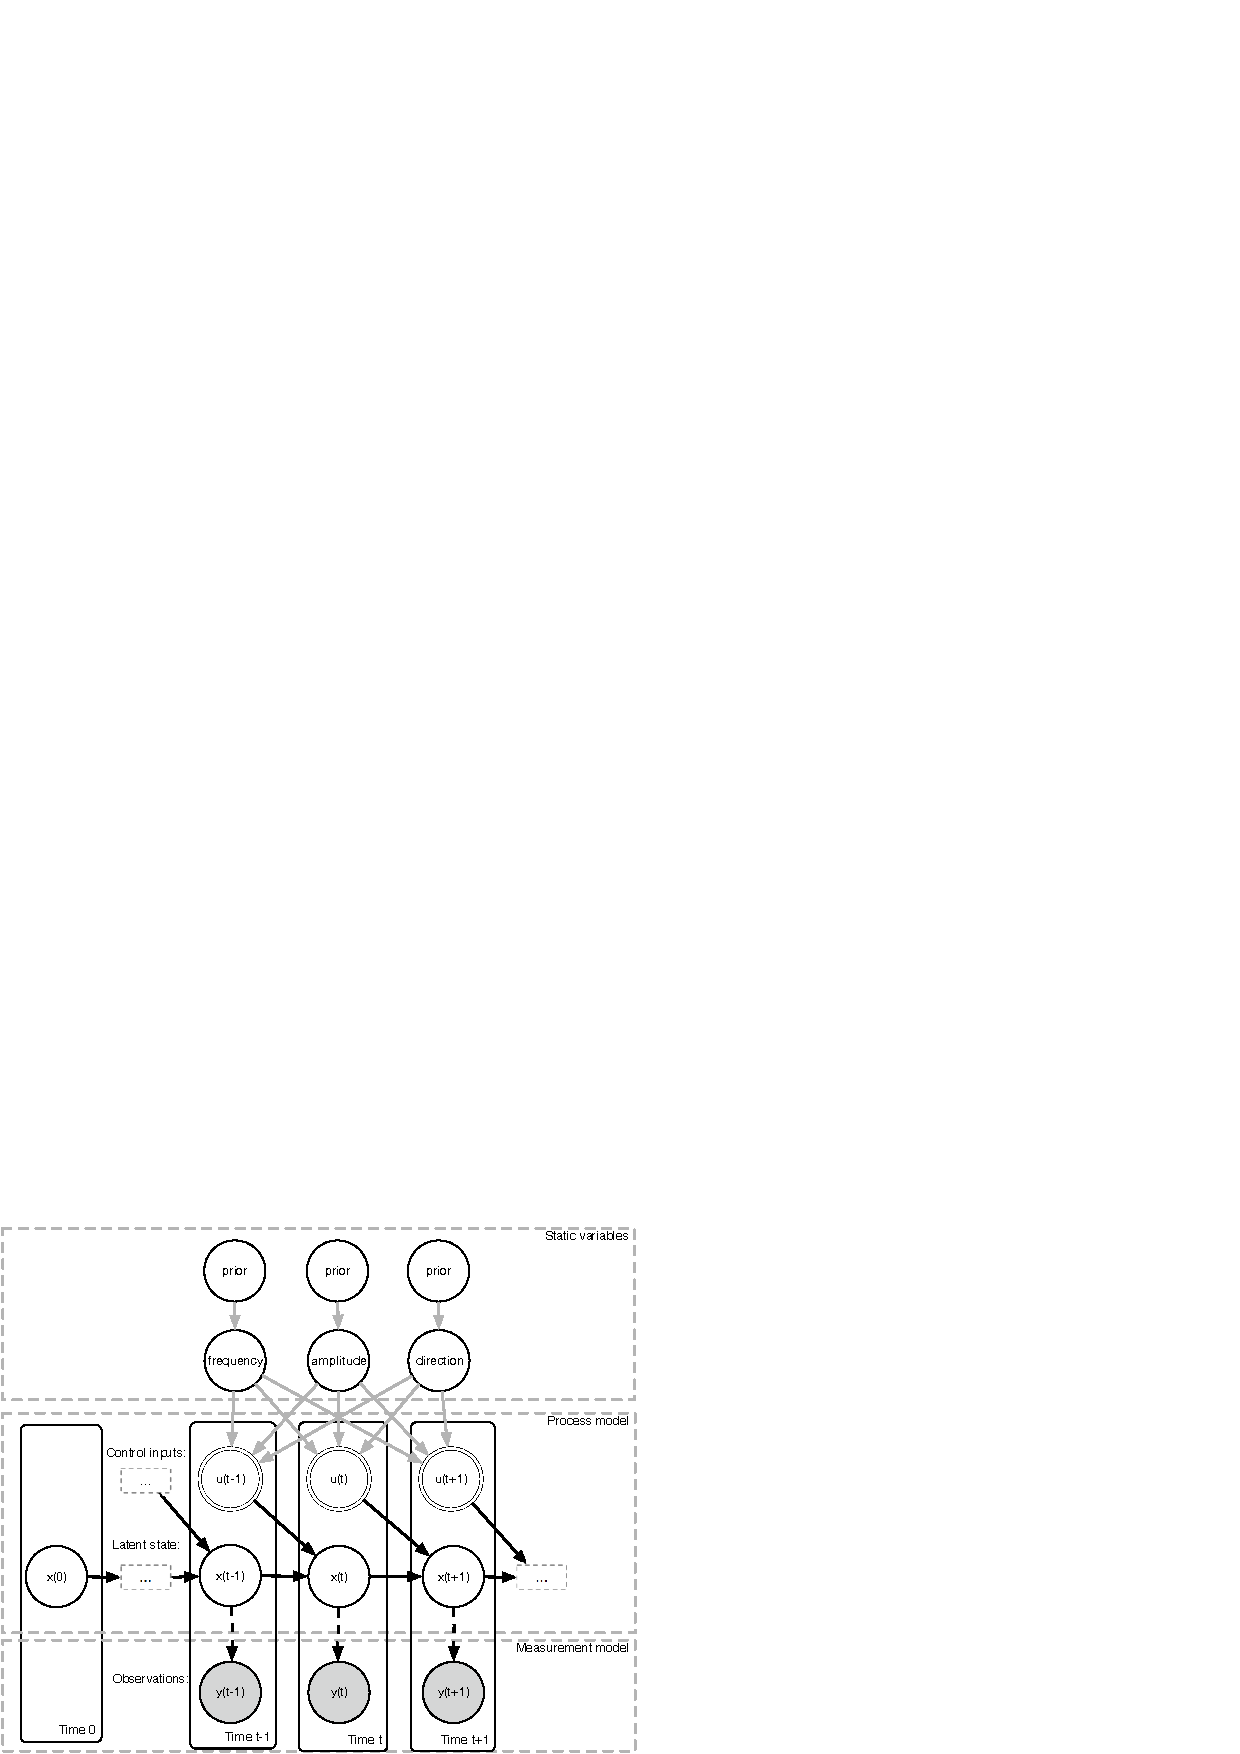
\includegraphics{diagrams/dynamic-belief-network-inference-2.pdf}
\caption{\label{fig:graphical-model-control}Graphical model extended with
hierarchical model for self-initiated movements.}
\end{figure}

\section{\texorpdfstring{\textbf{BIS
HIER.}}{BIS HIER.}}\label{bis-hier.}

\section{TODO: Modelling questions}\label{todo-modelling-questions}

Note the the vestibular senspry input may be the result of a
superposition of multiple generative source; the afferent signals,
measuring head velocity, may be caused by a multitude of processes
(active head turn, unintentional body sway, perturbative external forcec
(wind), etc.). The brain must treat these resulting head movements
differently; active head turn may be goal-directed, with the aim of
directing the gaze toward a target. In this case, no compensatory action
os desired in order to counteract the movement. This would be
counterproductive. However, in order to maintian postural stability, the
brain must compensate for all movement that is not gol-directed,
i.e.~does not occur as a result of \enquote{planned} active motion.
These components may be separated either at the level of the outcome
variable (sensory signal), or at the level of the latent state
variables. The latter amounts ot a latent decomposition.

\begin{quote}
Estimated velocity due to active/passive movement must be trated
differently. Sensory signals due to active motion (re-afference) can be
viewed as being cause by known explanatory variables, or as intervention
effects.
\end{quote}

\begin{quote}
discuss ({\textbf{???}}) (artificial velcoity vector)
\end{quote}

\begin{itemize}
\tightlist
\item
  Connecting higher cognition to sensory inference:

  \begin{itemize}
  \tightlist
  \item
    imagery uses a similar generative model (copied from sensory model),
    then what is it doing?
  \item
    \textbf{how does mental simulation work? When we propose a mental
    simulation, what does this actually mean? When we propose that
    simulation re-uses the circuit for sensory inference, which parts
    are actually required? Do we need the data? Surely not. NO, we need
    the generative model that is used for on-line inference, but we
    should not perform inference with it. ON the contrary, we should
    avoid inference at all costs, instead running a Monte Carlo
    simulation with the generative model, i.e.~just evolving the
    evolution of the dynamical system according to the transition prior
    (sampling from the proposal distribution).}
  \item
    mental simulation allows us to answer \enquote{what if}
    (counterfactual) queries in a generative model. Why should this
    model be close to the sensory model? What if the senspry model
    changes? The twin model needs updating.
  \item
    If mental simulation interferes with sensory inference: how?
  \item
    \textbf{If we want to model higher level cognition as being
    connected to (grounded in) lower level sensory circuits, we can join
    both in a hierarchical graphical model.}
  \end{itemize}
\item
  Explain what tasks sensory inference must perform. Tasks the are
  particular to the modality that senses movements of the body. It needs
  to detect non-linearities, i.e.~non-stationary process. This means ist
  needs to detect the sudden onset of movements, or sudden direction
  changes. When these are passive and cannot be predicted , the best the
  system can hope for is to detect the changes as quickly as possible.
  When they are the result of active movement, they can be predicted.
  But they can also be anticipated due to knowledge from other sources,
  such as visual or verbal clues; if the knowledge is available, how
  does the system make use of it? Proposal distribution use for
  sequential importance sampling are notoriously difficult to design.
  The approach of sampling from the prior can be very inefficient, as
  when the process is not stationary, i.e.~in this case when there are
  sudden changes in acceleration, the likelihood can change abruptly,
  and the weights would become neglible for all particles. In certain
  cases, the filter cannot recover from this, and would completely
  misrepresent the data. We propose that the ability to anticipate must
  result in the construction (flexible) of a proposal distribution, and
  that interference between mental simulation and inference involves the
  proposal distribution.
\end{itemize}

\begin{quote}
Control input for predictions is used to \enquote{design} better
proposal distributions for inference.
\end{quote}

\begin{itemize}
\tightlist
\item
  Experimental results to be explained: Wertheim et al. (2001) report a
  cognitive suppression of otolith responses, based on participants'
  prior beliefs about possible motions.
\end{itemize}

\subsection{TODO: Contrast model with Merfeld
(2016)}\label{todo-contrast-model-with-merfeld-2016}

Merfeld's model claims: filtering is performed at a low level in order
to extract velocity (maybe peak velocity?) and then this estimate is
processed sub-optimally by low-pass filtering. The decision variable is
computed at a higher level and separate from the model that is invloved
in inference.

We propose that there is an alternaitve way of looking at this. What if
there a second system that \enquote{interprets} the data when sensory
inference using the 3-d state space representation alone is insufficent.
This model \enquote{steps in} when the uncertainty is high, and it is
this system that enables anticpation of non-stationarities, i.e.~onset
of sudden changes. This is derived from the system that allows us to
predict consequences of own actions through the use of a control input
obtained via a forward model from the cerebellum. This system would
traditionally be viewed as depending on the motor commands from commands
that are actually performed. Maybe this is more general, allowing the
brain to include an exogenous variable in order to predict as a control
input, i.e.~this can also include \enquote{covert} actions. This
flexible control of the exogenous input is actually necessary for
planning, etc. Flexible control of input means: the ability to clamp
nodes, i.e.~to fix nodes at certain values. Without the ability to clamp
higher-level node, the inference model can only be used inflexibly for
inference. The whole idea is based on the fact that higher level
knowledge and beliefs can influence our perception, and this is
especially true for vestibular signals, which are highly ambiguous, and
require prior knowledge for disambiguation and interpretation. Actually,
we should implement something similar to (Hamrick et al., n.d.): a
metacontroller, which chooses either the low-level module, or when this
is unable to deal with the problem, a higher level module. This higher
level module introduces additional information about the problem,
e.g.~information obtained by verbal instructions, or a bias. FOr
example, the instructions: \enquote{choose right when uncertain} should
lead participants to implement use this strategy. In other words, when
you are certain, base you choice on your low level sensory inference,
but when uncertain use other information, such as task demands. Surely
we can design a better experiment than this, though?

Implement the above ideas in a figure, showing the two approaches, and
differences, especially for predictions about future data.

\subsection{TODO: Simulations}\label{todo-simulations}

Show that when fit to the same data, a model implementing a control
provides substantially better fit, as measured by log-likelihood, when
compared to 3-d state space model (basic model) {[}think of better names
for models{]}. This is almost trivial; but show it like this: under the
assumption that the agent knows the precise timing (onset) of motion,
and the functional form (sinusiodal acceleration), all the agent needs
to assume is: \{A, direction, frequency\}. Show that performance is
substantially better if agent has priors for A, direction (maybe
ignoring f, or vice versa: ignore A, and put priors on f, might be
better). Then draw A (or f) from a distribution, and run inference using
control model. Sampling A from prior distribution means: the agent has
imperfect knowledge about its amplitude of motion.

This improvement in inference is only better when the proposal
distribution is well-specified; for a mis-specified model, the
performance can be dramatically worse.

We claim: interference effects arise when participant's wrongly use a
control (predictive model or \textbf{anticipation model}) using motion
paramters used for mental simulation during subsequent inference. This
use of higher level priors has the same (similar) effect as
anticipation.

\section{An investigation of various priors and
predictions}\label{an-investigation-of-various-priors-and-predictions}

Here, we identify the various forms of predictive processing in the
context of real-time sensory inference using SMC

\begin{itemize}
\tightlist
\item
  Related to filtering algorithm
\item
  Higher-level priors: The process model determines the kind of motion
  that is expected. Call this \emph{hypothesis-driven} sensory
  inference. It implements expectation on longer time-scales.
\end{itemize}

Show a table demonstrating the difference between:

\begin{itemize}
\tightlist
\item
  prediction: 1-step ahead during inference
\item
  expectation: higher level priors
\end{itemize}

The brain implements multiple priors:

\begin{itemize}
\tightlist
\item
  ability to select type of motion
\item
  parameters of the motion
\end{itemize}

\section{Various sources of
interference}\label{various-sources-of-interference}

Interference is interesting in its own right. It is important to
understand how and why this should occur. Furthermore, we propose that
gaining a better understanding of this will allow us to better
understand the nature of \enquote{thinking} as mental simulation.

Interference is rather surprising; if the goal is to perform simulation
without incorporating the data, then we should run a Monte Carlo
simulation. Why should this interfere with sensory inference perform by
a particle filter? We propose that the answer is in the shared
generative model.

Here, we identify various sources of interference (2-way) between
thought (higher-level cognition) and lower-level sensory processing.
This interference can be either due to low-level influences in sensory
inference, due to priors on higher-level parameters, choice of process
model (false expectations of certain type of motion). This is shown by
model simulations.

\begin{itemize}
\item
  Model mis-specification: If an observer uses a strong higher level
  prior, i.e.~the wrong direction, this means that the data may be
  completely mis-interpreted. (call this: the effect of inappropriate
  priors (Schwabe \& Blanke, 2008))
\item
  Re-use of same generative model: This may lead to leakage,
  i.e.~inadvertently incorporating sensory evidence
\item
  Decision-making: The interference may be explained in terms of
  higher-level perceptual decision-making mechanisms

  \begin{itemize}
  \tightlist
  \item
    evidence accumulation
  \item
    bias (Starting point)
  \end{itemize}
\end{itemize}

\subsection{Summary}\label{summary}

Interference may the result of either:

\begin{enumerate}
\def\labelenumi{\arabic{enumi})}
\tightlist
\item
  mis-specified proposal distribution: inappropriate priors, or wrong
  type of motion or
\item
  biased decision-making
\end{enumerate}

We should be able to investigate which by applying cognitive process
models that explain response times and choices.

\section{Simulations}\label{simulations}

\begin{quote}
Should we have a separate simulations section, or should the simulations
be distributed? \#\# Model specifications
\end{quote}

\subsection{Monte Carlo simulation}\label{monte-carlo-simulation}

Show dynamics when simulating using various proposal distributions
implementing various natural head motions:

\begin{itemize}
\tightlist
\item
  turning left
\item
  shaking head quickly
\item
  shaking head slowly (communicative gesture)
\end{itemize}

\subsection{Expectations based on higher level
priors}\label{expectations-based-on-higher-level-priors}

In our model, there is no difference between modelling active
self-motion, and an anticipation of passive self-motion due to
predictable external forces. This is a testable hypothesis.

\subsection{Model mis-specification}\label{model-mis-specification}

\subsubsection{Inappropriate priors}\label{inappropriate-priors}

\subsubsection{Wrong type of motion
model}\label{wrong-type-of-motion-model}

For example, expect shaking instead of head turn

\section{General Discussion}\label{general-discussion}

The main results of this study are:

\begin{itemize}
\item
  place the emerging field of vestibular cognition with a framework for
  dynamic probabilistic inference and draw links to established models
  of sensory processing
\item
  interpret result from vestibular cognition studies showing
  interference between thought and perception as being the result of
  biased sensory processing. This interference can be either due to
  low-level influences in sensory inference, due to priors on
  higher-level parameters, choice of process model (false expectations
  of certain type of motion). This is shown by model simulations.
\item
  A further possibility for interference is a bias introduced in the
  decision-making process (discuss potential model of decision-making
  based on sequential Bayes factor and contrast with (Merfeld, Clark,
  Lu, \& Karmali, 2016).)
\end{itemize}

\subsection{A comparison with previous
models}\label{a-comparison-with-previous-models}

Unfortunately, there aren't many, but see (Hiatt, Trafton, Harrison, \&
Schultz, 2004): imagined motion through space vs.~rotating contents of
visual buffer

\subsection{What is the difference between predicting and
imagining?}\label{what-is-the-difference-between-predicting-and-imagining}

Imagining can be described as counterfactual inference (Krishnan,
Shalit, \& Sontag, 2015). Imagined motion (for planning,
decision-making, perspective transformations) is performed under
counterfactual assumptions. Predictions/anticipation is performed under
factual assumptions.

\subsection{Support for our model:}\label{support-for-our-model}

\begin{itemize}
\tightlist
\item
  Nigmatullina
\item
  Wertheim (Grabherr, Cuffel, Guyot, \& Mast, 2011) showed that patients
  with bilateral or unilateral vestibular loss show impaired ability to
  mentally transform images of bodies and body parts.
\end{itemize}

\subsection{Neuronal implementation}\label{neuronal-implementation}

(Lopez \& Blanke, 2011; Lopez, Blanke, \& Mast, 2012) (Klingner, Axer,
Brodoehl, \& Witte, 2016) (Eulenburg, Müller-Forell, \& Dieterich, 2012)

\subsubsection{Sensory gating}\label{sensory-gating}

(Gale et al., 2016)

\subsubsection{Head direction cells}\label{head-direction-cells}

Head direction cells are thought to integrate signals of vestibular
origin to maintain a signal of cumulative rotation (reviewed in Taube
(2007) and are found in many brain areas, including the postsubiculum,
retrosplenial cortex, thalamus, lateral mammillary nucleus, dorsal
tegmental nucleus, striatum and entorhinal cortex (Cullen, 2014). This
may be necessary in order to mentally simulate being in another
position, i.e.~the brain apparently needs to simulate the n-step
dynamics of its motion through space. Why is this? Because vestibular
connections make a major contribution to spatial orientation;
information about the position in space obtained through the vestibular
sensory system is computed by integrating velocity over time.

\begin{itemize}
\item
  mental simulation cannot just re-use the state used in sensory
  inference, because the velocity is fed to the head direction cells.
  The brain would get confused
\item
  directional signal is not just a simple integration of velocity
  signals from the vestibular system
\item
  signals from motor efferecence copy or proprioceptive systems appear
  to be crucial for updating the preferred firing direction over time
\item
  Forward model for computing anticpation-related control input may
  reside in the cerebellum. THe cerebellum may be involved in imagined
  movemeent, or is it just for actions that are actually performed?
\end{itemize}

\subsection{Testable hypotheses}\label{testable-hypotheses}

Show a table of testable hypotheses

\section{Summary and conclusions}\label{summary-and-conclusions}

\section{Acknowledgements}\label{acknowledgements}

\newpage

\section{References}\label{references}

\setlength{\parindent}{-0.5in} \setlength{\leftskip}{0.5in}

\hypertarget{refs}{}
\hypertarget{ref-Andrieu:2010gc}{}
Andrieu, C., Doucet, A., \& Holenstein, R. (2010). Particle Markov chain
Monte Carlo methods. \emph{Journal of the Royal Statistical Society:
Series B (Statistical Methodology)}, \emph{72}(3), 269--342.

\hypertarget{ref-Baker:2009kx}{}
Baker, C. L., Saxe, R., \& Tenenbaum, J. B. (2009). Action understanding
as inverse planning. \emph{Cognition}, \emph{113}(3), 329--349.

\hypertarget{ref-Battaglia:2013fm}{}
Battaglia, P. W., Hamrick, J. B., \& Tenenbaum, J. B. (2013). Simulation
as an engine of physical scene understanding. \emph{Proceedings of the
National Academy of Sciences of the United States of America},
\emph{110}(45), 18327--18332.

\hypertarget{ref-Beveridge:2013gx}{}
Beveridge, M. E. L., \& Pickering, M. J. (2013). Perspective taking in
language: integrating the spatial and action domains. \emph{Frontiers in
Human Neuroscience}, \emph{7}.

\hypertarget{ref-Bishop:2006ui}{}
Bishop, C. M. (2006). \emph{Pattern Recognition and Machine Learning}.
Springer Verlag.

\hypertarget{ref-Borah:1988fd}{}
Borah, J., Young, L. R., \& Curry, R. E. (1988). Optimal Estimator Model
for Human Spatial Orientation. \emph{Annals of the New York Academy of
Sciences}, \emph{545}(1), 51--73.

\hypertarget{ref-Botvinick:2012fe}{}
Botvinick, M. M., \& Toussaint, M. (2012). Planning as inference.
\emph{Trends in Cognitive Sciences}, \emph{16}(10), 485--488.

\hypertarget{ref-Carriot:2014fv}{}
Carriot, J., Jamali, M., Chacron, M. J., \& Cullen, K. E. (2014).
Statistics of the vestibular input experienced during natural
self-motion: implications for neural processing. \emph{The Journal of
Neuroscience : The Official Journal of the Society for Neuroscience},
\emph{34}(24), 8347--8357.

\hypertarget{ref-Clark:2012vf}{}
Clark, A. (2012). Whatever Next? Predictive Brains, Situated Agents, and
the Future of Cognitive Science. \emph{Behavioral and Brain Sciences}.

\hypertarget{ref-Crapse:2008jc}{}
Crapse, T. B., \& Sommer, M. A. (2008). Corollary discharge across the
animal kingdom. \emph{Nature Reviews Neuroscience}, \emph{9}(8),
587--600.

\hypertarget{ref-CreemRegehr:2013kx}{}
Creem-Regehr, S. H., Gagnon, K. T., Geuss, M. N., \& Stefanucci, J. K.
(2013). Relating spatial perspective taking to the perception of other's
affordances: providing a foundation for predicting the future behavior
of others. \emph{Frontiers in Human Neuroscience}, \emph{7}, 596.

\hypertarget{ref-Cullen:2014gx}{}
Cullen, K. E. (2014). The neural encoding of self-generated and
externally applied movement: implications for the perception of
self-motion and spatial memory. \emph{Frontiers in Integrative
Neuroscience}, \emph{7}, 108.

\hypertarget{ref-Cullen:2009dc}{}
Cullen, K. E., Brooks, J. X., \& Sadeghi, S. G. (2009). How actions
alter sensory processing: reafference in the vestibular system.
\emph{Annals of the New York Academy of Sciences}, \emph{1164}, 29--36.

\hypertarget{ref-Deroualle:2014ho}{}
Deroualle, D., \& Lopez, C. (2014). Toward a vestibular contribution to
social cognition. \emph{Frontiers in Integrative Neuroscience},
\emph{8}.

\hypertarget{ref-Deroualle:2015gk}{}
Deroualle, D., Borel, L., Devèze, A., \& Lopez, C. (2015). Changing
perspective: The role of vestibular signals. \emph{Neuropsychologia},
\emph{79}, 175--185.

\hypertarget{ref-Doucet:2009us}{}
Doucet, A., \& Johansen, A. M. (2009). A tutorial on particle filtering
and smoothing: Fifteen years later. \emph{Handbook of Nonlinear
Filtering}.

\hypertarget{ref-Doucet:2000bh}{}
Doucet, A., Godsill, S., \& Andrieu, C. (2000). On sequential Monte
Carlo sampling methods for Bayesian filtering. \emph{Statistics and
Computing}, \emph{10}(3), 197--208.

\hypertarget{ref-Ellis:2017fg}{}
Ellis, A. W., \& Mast, F. W. (2017). Toward a Dynamic Probabilistic
Model for Vestibular Cognition. \emph{Frontiers in Psychology},
\emph{8}.

\hypertarget{ref-zuEulenburg:2012bh}{}
Eulenburg, P. zu, Müller-Forell, W., \& Dieterich, M. (2012). On the
recall of vestibular sensations. \emph{Brain Structure and Function},
\emph{218}(1), 255--267.

\hypertarget{ref-Falconer:2012cl}{}
Falconer, C. J., \& Mast, F. W. (2012). Balancing the mind: vestibular
induced facilitation of egocentric mental transformations.
\emph{Experimental Psychology}, \emph{59}(6), 332--339.

\hypertarget{ref-Gale:2016cx}{}
Gale, S., Prsa, M., Schurger, A., Gay, A., Paillard, A., Herbelin, B.,
\ldots{} Blanke, O. (2016). Oscillatory neural responses evoked by
natural vestibular stimuli in humans. \emph{Journal of Neurophysiology},
\emph{115}(3), 1228--1242.

\hypertarget{ref-Gambi:2015gv}{}
Gambi, C., \& Pickering, M. J. (2015). Predicting and imagining
language. \emph{Language}.

\hypertarget{ref-Gardner:2016kd}{}
Gardner, M. R., Stent, C., Mohr, C., \& Golding, J. F. (2016). Embodied
perspective-taking indicated by selective disruption from aberrant self
motion. \emph{Psychological Research}, 1--10.

\hypertarget{ref-Goodman:2016go}{}
Goodman, N. D., \& Frank, M. C. (2016). Pragmatic Language
Interpretation as Probabilistic Inference. \emph{Trends in Cognitive
Sciences}, \emph{20}(11), 818--829.

\hypertarget{ref-Grabherr:2011ej}{}
Grabherr, L., Cuffel, C., Guyot, J.-P., \& Mast, F. W. (2011). Mental
transformation abilities in patients with unilateral and bilateral
vestibular loss. \emph{Experimental Brain Research}, \emph{209}(2),
205--214.

\hypertarget{ref-Grabherr:2008kk}{}
Grabherr, L., Nicoucar, K., Mast, F. W., \& Merfeld, D. (2008).
Vestibular thresholds for yaw rotation about an earth-vertical axis as a
function of frequency. \emph{Experimental Brain Research. Experimentelle
Hirnforschung. Expérimentation cérébrale}, \emph{186}(4), 677--681.

\hypertarget{ref-Griffiths:2012ii}{}
Griffiths, T. L., Vul, E., \& Sanborn, A. N. (2012). Bridging levels of
analysis for probabilistic models of cognition. \emph{Current Directions
in Psychological Science}.

\hypertarget{ref-Grush:2004wx}{}
Grush, R. (2004). The emulation theory of representation: motor control,
imagery, and perception. \emph{The Behavioral and Brain Sciences},
\emph{27}(3), 377--96--discussion396--442.

\hypertarget{ref-Hamrick:2014wq}{}
Hamrick, J. B., \& Griffiths, T. L. (2014). What to simulate? Inferring
the right direction for mental rotation. \emph{CogSci}.

\hypertarget{ref-Hamrick:8oFH5gP_}{}
Hamrick, J. B., Ballard, A. J., Pascanu, R., Vinyals, O., Hees, N., \&
Battaglia, P. W. (n.d.). Metacontrol For Adaptive Imagination-Based
Optimization. Retrieved from
\url{https://openreview.net/pdf?id=Bk8BvDqex}

\hypertarget{ref-Hiatt:2004tv}{}
Hiatt, L. M., Trafton, J. G., Harrison, A. M., \& Schultz, A. C. (2004).
A Cognitive Model for Spatial Perspective taking. In \emph{Proceedings
of the sixth international conference on cognitive modeling} (pp.
354--355).

\hypertarget{ref-Karmali:2012cv}{}
Karmali, F., \& Merfeld, D. (2012). A distributed, dynamic, parallel
computational model: the role of noise in velocity storage.
\emph{Journal of Neurophysiology}, \emph{108}(2), 390--405.

\hypertarget{ref-Kemp:2007eo}{}
Kemp, C., Perfors, A., \& Tenenbaum, J. B. (2007). Learning
overhypotheses with hierarchical Bayesian models. \emph{Developmental
Science}, \emph{10}(3), 307--321.

\hypertarget{ref-Klingner:2016ia}{}
Klingner, C. M., Axer, H., Brodoehl, S., \& Witte, O. W. (2016). Vertigo
and the processing of vestibular information: A review in the context of
predictive coding. \emph{Neuroscience and Biobehavioral Reviews},
\emph{71}, 379--387.

\hypertarget{ref-Koller:2009ty}{}
Koller, D., \& Friedman, N. (2009). \emph{Probabilistic Graphical
Models}. MIT Press.

\hypertarget{ref-Krishnan:2015wr}{}
Krishnan, R. G., Shalit, U., \& Sontag, D. (2015). Deep Kalman Filters.
Retrieved from \url{http://arxiv.org/abs/1511.05121}

\hypertarget{ref-Kwisthout:2016fx}{}
Kwisthout, J., Bekkering, H., \& Rooij, I. van. (2016). To be precise,
the details don't matter: On predictive processing, precision, and level
of detail of predictions. \emph{Brain and Cognition}.

\hypertarget{ref-Laurens:2006be}{}
Laurens, J., \& Droulez, J. (2007). Bayesian processing of vestibular
information. \emph{Biological Cybernetics}, \emph{96}(4), 389--404.

\hypertarget{ref-Lenggenhager:2008et}{}
Lenggenhager, B., Lopez, C., \& Blanke, O. (2008). Influence of galvanic
vestibular stimulation on egocentric and object-based mental
transformations. \emph{Experimental Brain Research}, \emph{184}(2),
211--221.

\hypertarget{ref-Lopez:2011cc}{}
Lopez, C., \& Blanke, O. (2011). The thalamocortical vestibular system
in animals and humans. \emph{Brain Research Reviews}, \emph{67}(1-2),
119--146.

\hypertarget{ref-Lopez:2012ek}{}
Lopez, C., Blanke, O., \& Mast, F. W. (2012). The human vestibular
cortex revealed by coordinate-based activation likelihood estimation
meta-analysis. \emph{Neuroscience}, \emph{212}, 159--179.

\hypertarget{ref-Lucas:2010tu}{}
Lucas, C. G., \& Griffiths, T. L. (2010). Learning the form of causal
relationships using hierarchical Bayesian models. \emph{Cognitive
Science}.

\hypertarget{ref-PaulRMacNeilage:2008bv}{}
MacNeilage, P. R., Ganesan, N., \& Angelaki, D. E. (2008). Computational
approaches to spatial orientation: from transfer functions to dynamic
Bayesian inference. \emph{Journal of Neurophysiology}, \emph{100}(6),
2981--2996.

\hypertarget{ref-Merfeld:2011fs}{}
Merfeld, D. (2011). Signal detection theory and vestibular thresholds:
I. Basic theory and practical considerations. \emph{Experimental Brain
Research. Experimentelle Hirnforschung. Expérimentation cérébrale},
\emph{210}(3-4), 389--405.

\hypertarget{ref-Merfeld:2016il}{}
Merfeld, D., Clark, T. K., Lu, Y. M., \& Karmali, F. (2016). Dynamics of
individual perceptual decisions. \emph{Journal of Neurophysiology},
\emph{115}(1), 39--59.

\hypertarget{ref-Merfeld:1999cg}{}
Merfeld, D., Zupan, L. H., \& Peterka, R. J. (1999). Humans use internal
models to estimate gravity and linear acceleration. \emph{Nature},
\emph{398}(6728), 615--618.

\hypertarget{ref-Moulton:2009ij}{}
Moulton, S. T., \& Kosslyn, S. M. (2009). Imagining predictions: mental
imagery as mental emulation. \emph{Philosophical Transactions of the
Royal Society of London Series B, Biological Sciences},
\emph{364}(1521), 1273--1280.

\hypertarget{ref-Murphy:2012ua}{}
Murphy, K. P. (2012). \emph{Machine Learning}. MIT Press.

\hypertarget{ref-Nigmatullina:2015gh}{}
Nigmatullina, Y., Arshad, Q., Wu, K., Seemungal, B. M., Bronstein, A.
M., \& Soto, D. (2015). How imagery changes self-motion perception.
\emph{Neuroscience}, \emph{291}, 46--52.

\hypertarget{ref-Pearl:1988wz}{}
Pearl, J. (1988). \emph{Probabilistic Reasoning in Intelligent Systems}.
Morgan Kaufmann.

\hypertarget{ref-Penny:2013iv}{}
Penny, W. D., Zeidman, P., \& Burgess, N. (2013). Forward and backward
inference in spatial cognition. \emph{PLoS Computational Biology},
\emph{9}(12), e1003383.

\hypertarget{ref-Perfors:2011ex}{}
Perfors, A., Tenenbaum, J. B., Griffiths, T. L., \& Xu, F. (2011). A
tutorial introduction to Bayesian models of cognitive development.
\emph{Cognition}, \emph{120}(3), 302--321.

\hypertarget{ref-Pezzulo:2013iy}{}
Pezzulo, G., Iodice, P., Ferraina, S., \& Kessler, K. (2013). Shared
action spaces: a basis function framework for social re-calibration of
sensorimotor representations supporting joint action. \emph{Frontiers in
Human Neuroscience}, \emph{7}, 800.

\hypertarget{ref-Pickering:2014bo}{}
Pickering, M. J., \& Clark, A. (2014). Getting ahead: forward models and
their place in cognitive architecture. \emph{Trends in Cognitive
Sciences}, \emph{18}(9), 451--456.

\hypertarget{ref-Raphan:1979hn}{}
Raphan, T., Matsuo, V., \& Cohen, B. (1979). Velocity storage in the
vestibulo-ocular reflex arc (VOR). \emph{Experimental Brain Research},
\emph{35}(2).

\hypertarget{ref-Schwabe:2008ho}{}
Schwabe, L., \& Blanke, O. (2008). The vestibular component in
out-of-body experiences: a computational approach. \emph{Frontiers in
Human Neuroscience}, \emph{2}.

\hypertarget{ref-Selva:2012gsa}{}
Selva, P., \& Oman, C. M. (2012). Relationships between observer and
Kalman Filter models for human dynamic spatial orientation.
\emph{Journal of Vestibular Research : Equilibrium \& Orientation},
\emph{22}(2), 69--80.

\hypertarget{ref-Speekenbrink:2016kc}{}
Speekenbrink, M. (2016). A tutorial on particle filters. \emph{Journal
of Mathematical Psychology}.

\hypertarget{ref-Taube:2007fk}{}
Taube, J. S. (2007). The head direction signal: origins and
sensory-motor integration. \emph{Annual Review of Neuroscience},
\emph{30}, 181--207.

\hypertarget{ref-Tenenbaum:2011hd}{}
Tenenbaum, J. B., Kemp, C., Griffiths, T. L., \& Goodman, N. D. (2011).
How to grow a mind: statistics, structure, and abstraction.
\emph{Science}, \emph{331}(6022), 1279--1285.

\hypertarget{ref-Tian:2012ui}{}
Tian, X., \& Poeppel, D. (2012). Mental imagery of speech: linking motor
and perceptual systems through internal simulation and estimation.
\emph{Frontiers in Human Neuroscience}.

\hypertarget{ref-Wertheim:2001cb}{}
Wertheim, A. H., Mesland, B. S., \& Bles, W. (2001). Cognitive
suppression of tilt sensations during linear horizontal self-motion in
the dark. \emph{Perception}, \emph{30}(6), 733--741.

\hypertarget{ref-Wolpert:1998td}{}
Wolpert, D. M., \& Kawato, M. (1998). Multiple paired forward and
inverse models for motor control. \emph{Neural Networks : The Official
Journal of the International Neural Network Society}, \emph{11}(7-8),
1317--1329.


\clearpage
\renewcommand{\listtablename}{Table captions}
\listoftables

\clearpage
\renewcommand{\listfigurename}{Figure captions}
\listoffigures



\end{document}
